\documentclass[12pt,a4paper]{article}
%-----------------------------------------------------------------------------------------------------------------------------------------------------------------------------------------------       Package
\usepackage[utf8]{inputenc}
\usepackage[left=2.5cm, right=2.5cm, top=3.2cm, bottom=2cm, headsep=2.5cm]{geometry}
\usepackage{listings}
\usepackage{amsmath}
\usepackage{graphicx}
\usepackage{multirow}
\usepackage{natbib}

\usepackage{float}

%----- ABSTRACT

%----- En tête

\title{Reconstruction d'un tableau sans reflets à partir de photos prises sous des angles différents}
\date{16 Mai 2014}
\author{Théophile DALENS et Jean CAILLÉ}

\begin{document}
\maketitle

%------------------------------------------> SECTION Introduction
\section{Introduction}
Il devient aujourd'hui facile d'obtenir des photos de chefs-d'oeuvre dans un musée. Toutefois la présence de lumières couplés aux vernis et aux cadre en verres entraine sur la plupart des photos prises des reflets peu plaisants à l'oeil. En multipliant les points de vue, nous allons voir qu'il est possible de supprimer ces reflets et d'obtenir une photo proche de celle prise dans des conditions idéales.

%------------------------------------------> SECTION Méthode
\section{Méthode}

La méthode proposée par l'article ne s'attache pas à traiter le tableau sous l'angle de la reconnaissance d'image (reconnaitre par exemple les aplats de couleurs et supprimer les reflets à partir de cette information), mais uniquement grâce à des techniques génériques, permettant leur application sur la pluspart des tableaux. L'idée consiste à prendre plusieurs photos du même tableau sous différents angles. Les reflets ne dégraderons pas alors la même zone du tableau sur les différentes images et nous pourrons reconstruire à partir de ces images une image "virtuelle" sans reflets.\\

L'algorithme suggéré par l'article se décompose en deux parties. Tout d'abord, les images sont "recaléss" afin d'obtenir une perspective commune. Ainsi, les pixels des différentes images correspondent aux mêmes zones sur le tableaux, et il devient plus facile de reconstruire l'image corrigée. La seconde partie correspond justement à cette reconstructions. Plusieurs méthodes sont suggérées et nous nous sommes attachés à implémenter et comparer les différentes méthodes de fusion d'image proposées.

FIGURE - 3 ETAPES

%---------------------------------------------------> SUB SECTION Recalage des images
\subsection{Recalage des images}

Comme décrit plus haut, la première partie revient à "recaler" les images entre elles, c'est à dire simuler une perspective commune entre les photos. Sois nous pouvons nous attacher à modifier toutes les photos pour recaler l'image du tableau sur un rectangle donné, mais cela nécessite une connaissance \emph{a priori} des dimensions du tableau, que nous ne connaissons pas. Pour palier à ce problème, nous choisissons parmis les images de la peinture une photo dite de \emph{référence} et nous recadrerons les autres pour les afficher sous cette perspective.\\

Dans le cas où la caméra est idéale (modèle sténopé, pas de déformation dues à la lentille), et le tableau est parfaitement plan, la transormation permettant de recaler un tableau est une perspective. Nous n'avons pas eu besoin lors de nos traitement d'hypothèses supplémentaires.

%------------------------------------------------------------> SUB SUB SECTION Recalage manuel
\subsubsection{Recalage manuel}
Pour trouver la perspective liant deux images données, la solution la plus simple est de demander à l'utilisateur de cliquer sur 4 points communs entre les deux photos (par exemple les quatre coins du tableau). On obtient alors 2 quadrilatères quelconques, définis par les points ${p_i}_{i = 1...4}$ dans l'image de référence et ${p_i}_{i = 1...4}$ dans l'image que  l'on souhaite recaler.
On peut à partir ce ces points trouver une perspective permettant de passer du premier quadrilatère à l'autre, en effet, il existe en effet une et unique matrice $M$ en coordonées homogènes tel que

$$ \forall i \in \{1...4\}, q_i = M p_i $$

Une fois que nous avons trouvé la matrice $M$, il est possible de redresser l'image pour que les deux quadrilatères coincides, en appliquant la perspective définie par M. \\
Toutefois, il est peu probable que les valeurs de l'image de référence à échantilloner aient des coordonées entières (\emph{e.g.} des pixels). Nous devons donc pouvoir interpoler l'image de référence pour construire l'image redréssée. Plusieurs méthodes sont alors possible :
\paragraph{Interpolation au plus proche}
Pour trouver la valeur du pixel $(x,y)$ dans l'image de référence, on arrondi simplement les deux nombres pour tomber su un pixel. Cette méthode est simple à utiliser, mais moins précise que l'interpolation linéaire.

\paragraph{Interpolation Bilinéaire}
Dans cette méthode, pour trouver la valeur du pixel $(x,y)$, on observe les 4 valeur des pixels les plus proches et on interpole bilinéairement.

En pratique, nous avons choisi d'interpoller l'image de façon bilinéaire, plus précise et donc plus adaptée au travail de fusion qui viendra par la suite

\paragraph{Problème avec la méthode manuelle}

En pratique, cette méthode de recalage manuelle n'est pas utilisable pour plusieurs raisons. D'une part, le temps nécessaire pour définir les coins de chaques peinture est relativement long. D'autre part, la précision obtenue lors de nos test n'est pas suffisante pour l'étape suivante du traitement. En effet, l'utilisateur ne peux cliquer qu'avec une précision de quelques pixels au plus. Pour palier à ces problèmes, l'article suggère une solution plus automatisée, faisant appel à des descripteurs locaux.

\begin{figure}[H]
  \centering
  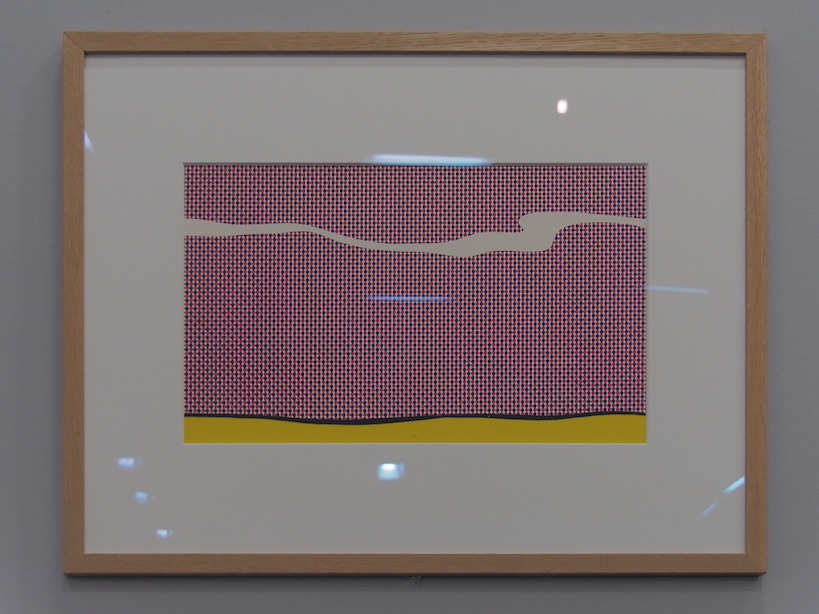
\includegraphics[width=0.45\textwidth]{Fig/User_reference.png}
  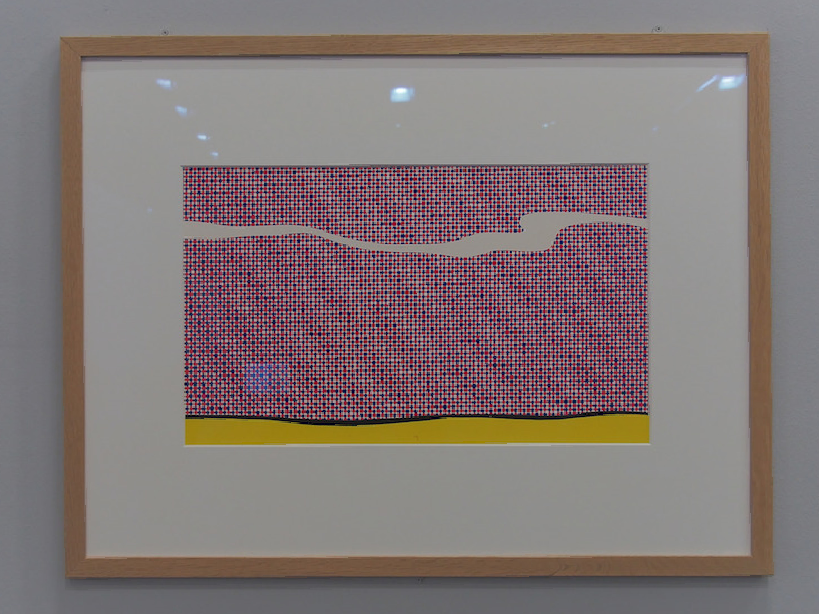
\includegraphics[width=0.45\textwidth]{Fig/User_fitted.png}\\ \vspace{0.1cm}
  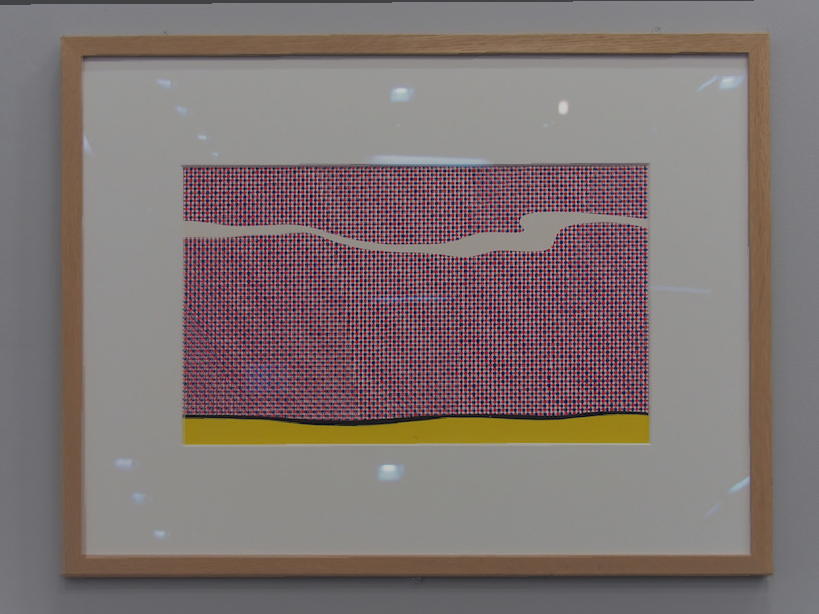
\includegraphics[width=0.45\textwidth]{Fig/User_average.png}

  \caption{En haut : Image de référence et image après recalage avec la méthode manuelle. En bas : Superposition des deux images. On observe des zones (particulièrement en bas à gauche) ou le recalage n'est pas bon.}
\end{figure}

%------------------------------------------------------------> SUB SUB SECTION Recalage automatique avec utilisation des  SIFT
\subsubsection{Recalage automatique avec utilisation des  SIFT}

Pour obtenir une précision sous-pixellique, nous utilisons des descripteurs locaux pour trouver des correspondances entre les deux image.

\paragraph{SIFT}
Les SIFT~\citep{lowe1999object}(Scale Invariant Feature Transform) sont des descripteurs locaux globalement inviariants aux changements de perspectives. Ils sont généralement utilisés pour détecter les correspondances entre des objets présent dans deux images différentes et sont donc très adaptés au problème actuel. Ils sont de plus invariants aux changements d'échelles et de luminosité, rendant plus robuste l'algorithme de recadrage.

FIGURE

\paragraph{Recherche de correspondances}
Nous extrayons de chaque image plusieurs centaines de SIFTs, auxquels sont associés leurs descripteurs. Nous recherchons ensuite des correspondances entre les images. Plusieurs algorithmes existent, mais le plus simple consiste à prendre pour chaque point de la première image le point le plus proche (dans l'espace des descripteurs) comme correspondant. Pour éviter d'obtenir un trop grand nombre de faux-positifs, un seuillage est effectué, nous permettant d'obtenir des correspondances point-à-point entre les deux images

\begin{figure}[H]
  \centering
  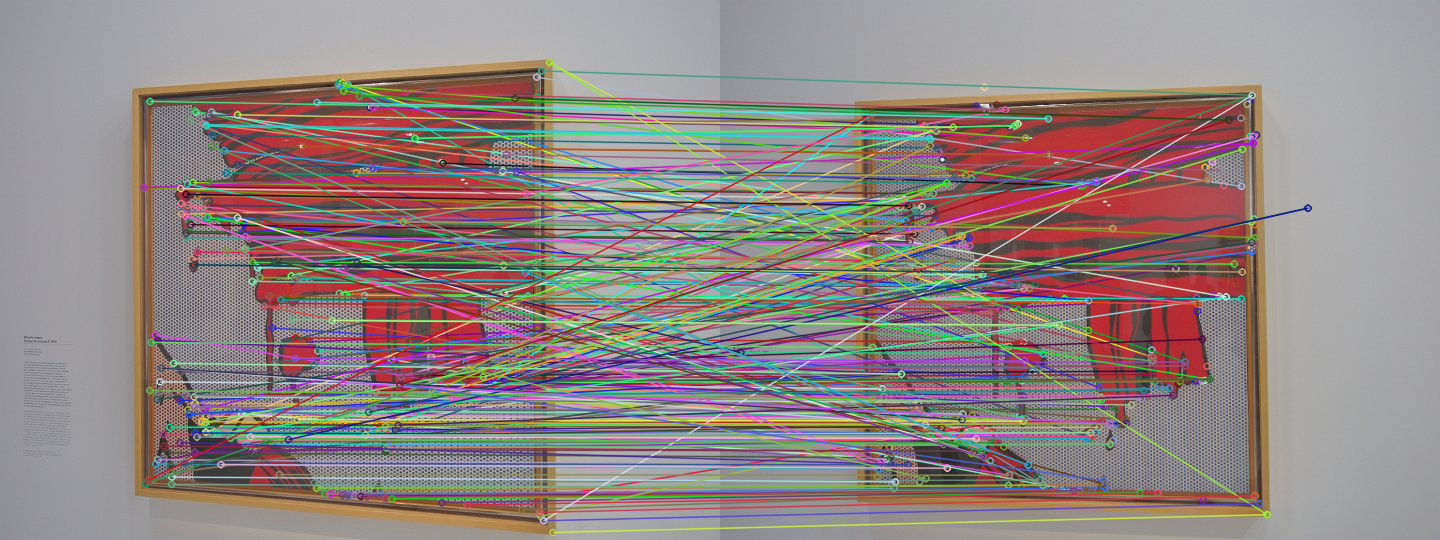
\includegraphics[width=0.75\textwidth]{Fig/sift_raw.png}
  \caption{Paires de descripteurs SIFT entre les deux images. Il existe encore un grand nombre de fausses-corresondances}
\end{figure}


\paragraph{RANSAC}
Il reste donc à trouver la matrice $M$ permettant de passer de l'image à recadre à l'image de référence. Contrairement au recalage manuel, il n'existe pas de tel matrice pour plus de quatre paires de points. Toutefois, si toutes les correspondances sont correctes (et il n'existe pas de faux-positifs), il est possible de trouver une matrice minimisant l'erreur $e$, par exemple par descente de gradient.

$$ e = \sum_{i = 1}^{n}\|p_i - Mq_i\|^2$$

Cependant, la présence de faux-positifs (c'est-à-dire des paires de points qui ne correspondent pas d'une image à l'autre), il est nécessaire d'employer un algorithme plus robuste pour trouver cette homographie. La méthode RANSAC~\citep{fischler1981random} permet à la fois de filtrer les bonnes correspondances et d'obtenirs cette homographie. Cet algorithme itératif sélectionne un sous-ensemble de descripteurs aléatoirement et marque ces correspondances comme "bonnes". On cherche ensuite l'homographie la plus adaptée à cet ensemble de point (en minimisant l'erreur $e$ par exemple), puis on cherche les correspondances qui sont "d'accord" avec cette homographie (celle pour lesquelles l'erreur résiduelle est inféiruer à un certain seuil). Si suffisement de paires sont en accord avec l'homographie trouvée, elle est conservée, sinon, l'algorithme est relancé avec une nouvelle initialisation aléatoire.

Cet algorithme est extrêment robuste et peut supporter un grand nombre de faux-positifs (jusqu'à 50\% dans certains cas). Toutefois, la convergence n'est pas forcément assurée. Il y'a également un certains nombres de paramètres dont les valeurs sont à ajuster en fonction du problèmes.

En pratique toutefois, et sur la pluspart des photos, l'algorithme de RANSAC permet de trouver une bonne correspondance entre les différentes images. 

\begin{figure}[H]
  \centering
  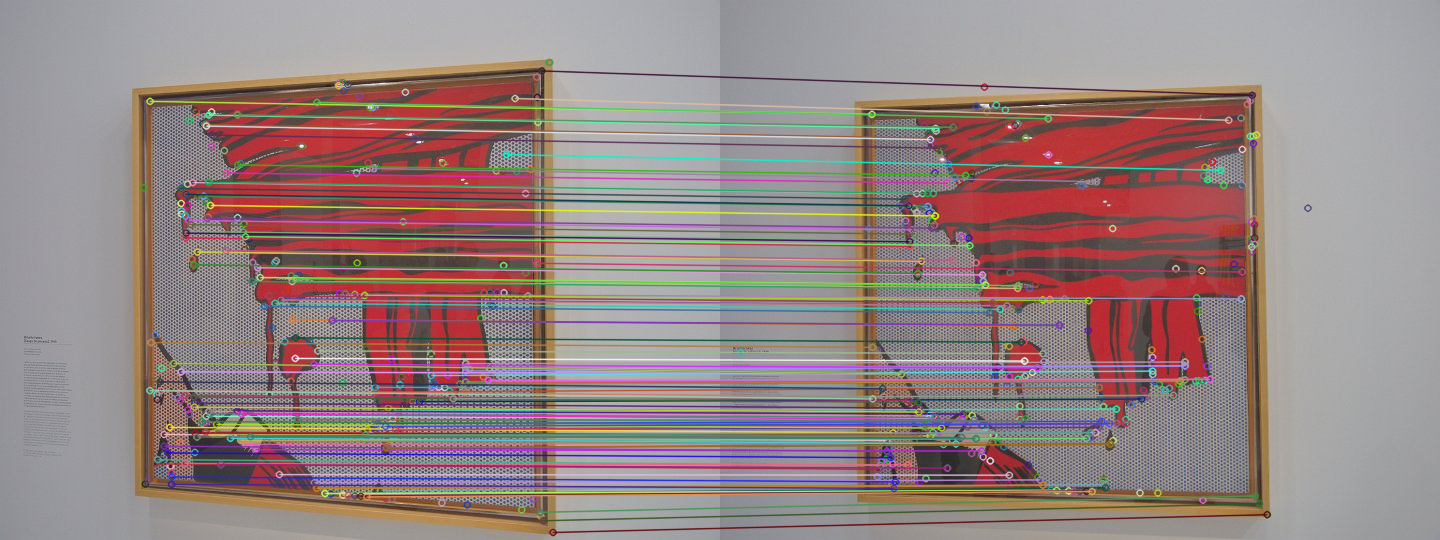
\includegraphics[width=0.75\textwidth]{Fig/sift_ransac.png}
  \caption{Paires de descripteurs SIFT estimés correctes par l'algorithme RANSAC et utilisés pour renconstruire la perspective}
\end{figure}


\begin{figure}[H]
  \centering
  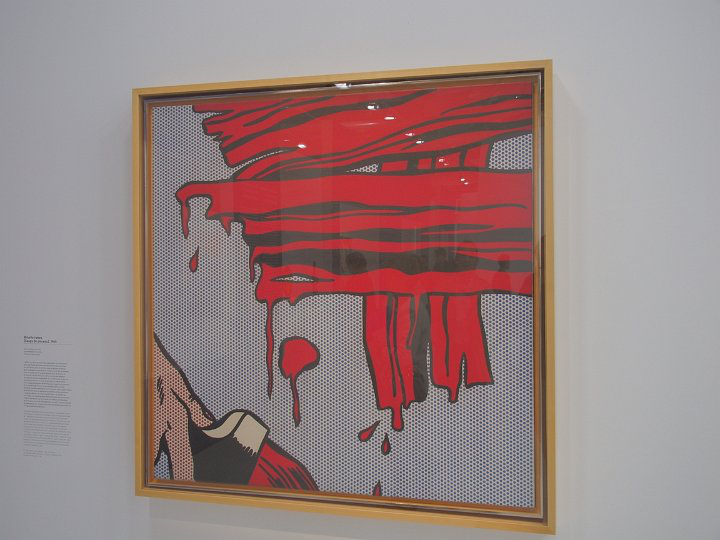
\includegraphics[width=0.30\textwidth]{Fig/working.png}
  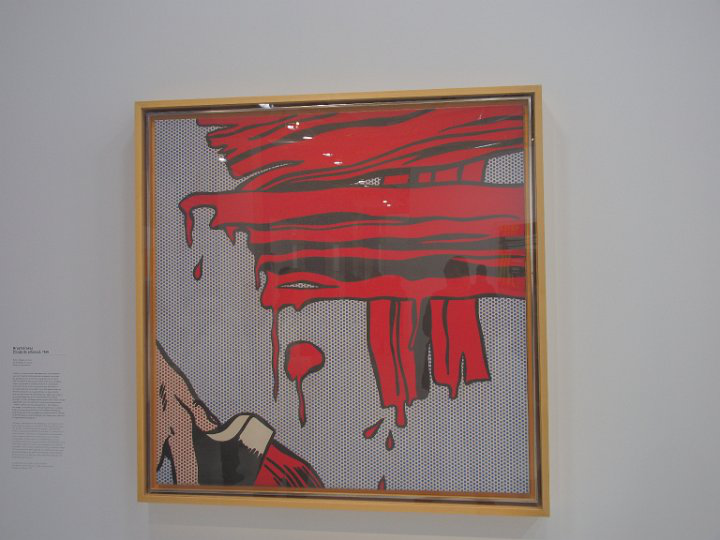
\includegraphics[width=0.30\textwidth]{Fig/reference_image.png}
  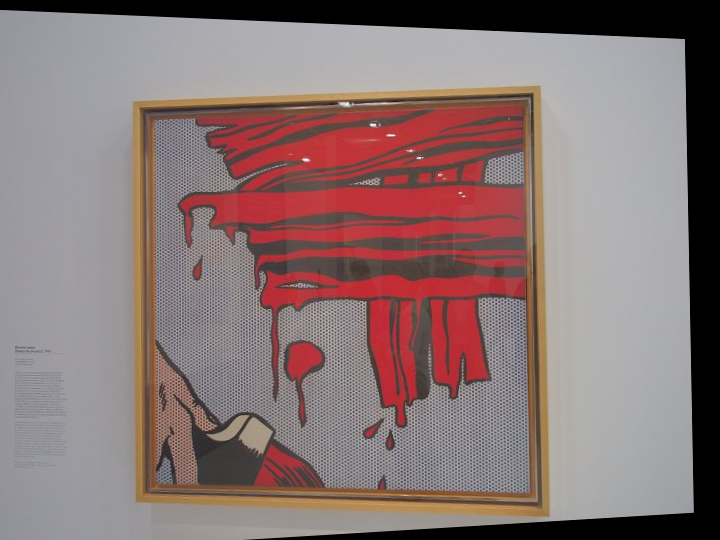
\includegraphics[width=0.30\textwidth]{Fig/fitted.png}

  \caption{A gauche : image de travail, au centre : image de référence, à droite : image de travail après recalage par rapport à l'image de référence. Noter la différence de position des reflets entre l'image de référence et l'image recalée}
\end{figure}

%------------------------------------------------------------> SUB SUB SECTION Amélioration
\subsubsection{Amélioration}

Plusieurs améliorations des méthodes proposées auparavant sont possibles, tant sur le modèle que sur la robustesse du système et du traitement des données

\paragraph{Prise en compte des déformations dues à la lentilles}
La méthode proposée ci dessus est suffisante pour la pluspart des améliorations, mais n'est pas parfaites, en effet, les déformations dues à la lentille de la caméra induise des imperfections dans les images. Une simple perspective ne peux pas corriger ces déformations, et le recalage n'est pas idéal.

\begin{figure}[H]
  \centering
  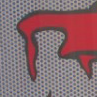
\includegraphics[width=0.45\textwidth]{Fig/Recalage_OK.png}
  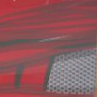
\includegraphics[width=0.45\textwidth]{Fig/Recalage_flou.png}
  \caption{Détails de la moyenne de l'image recalées et de l'image de référence. A gauche, le recalage est correcte et les contours sont nets. A droite, sur le bord de l'image, le recalage est moins bon, et les contours sont flous.}
\end{figure}

Pour palier à ce problème, l'article suggère un modèle prenant en compte les déformations dues à la lentille, et se basant sur un polynôme de degré 4 $P(x,y)$. Pour trouver ce polynôme, la matrice de perspective $M$ est obtenue par l'algorithme de RANSAC, puis les points en "accord" avec cette matrice au sens de RANSAC sont utilisés pour trouver les meilleurs coefficients du polynôme. La correction à appliquer à l'image est donc 

$$ q'_i = M q_i + P(q_i) $$

\paragraph{Amélioration de la robustesse de la méthode SIFT}
Sur plusieurs jeux d'images, la méthode SIFT n'a pas été adaptée, et proposait des recalages abberants, inuitilisable pour la fusion d'image.

\begin{figure}[H]
  \centering
  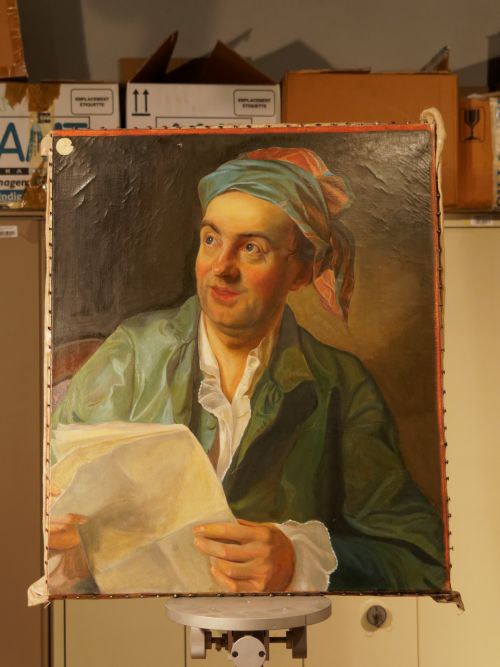
\includegraphics[width=0.25\textwidth]{Fig/error_reference.png}
  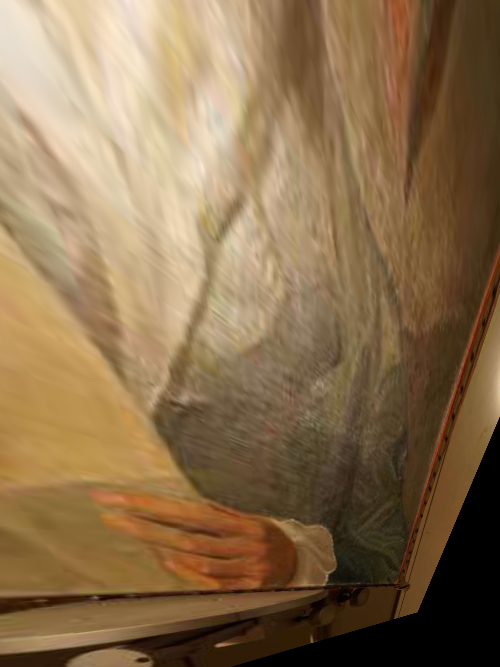
\includegraphics[width=0.25\textwidth]{Fig/error_fitted.png}
  \caption{Image de référence, et image inccorectement recalés}
\end{figure}

Deux solutions possibles peuvent venir à l'esprit. D'une part, nous pourrions rejeter automatiquement les images où le nombre de correspondances "bonnes" selon RANSAC est trop faible, et où le recalage n'est pas acceptable. D'autre part, nous pourrions demander à l'utilisateur d'indiquer grossièrement les coins du tableau. Ceci permet d'obtenir une approximation de la "bonne" perspective, et de restreindre la recherche par RANSAC à un espace plus petit.

\begin{figure}[H]
  \centering
  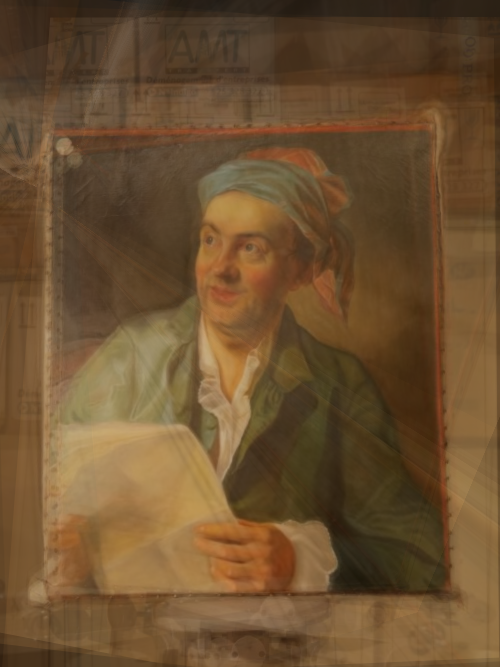
\includegraphics[width=0.45\textwidth]{Fig/merge_no_rejection.png}
  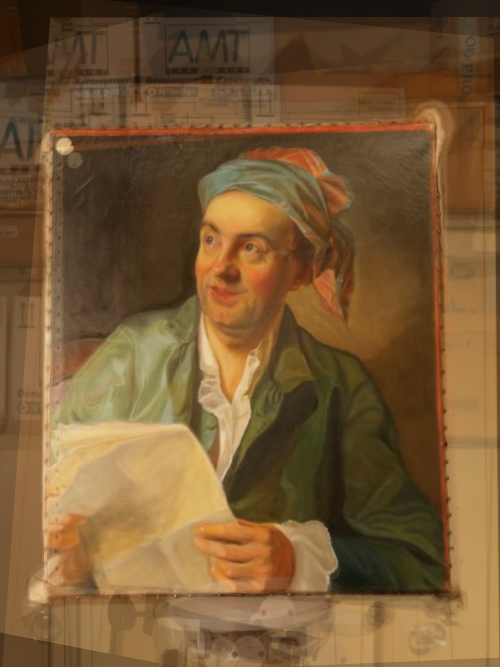
\includegraphics[width=0.45\textwidth]{Fig/merge_rejection.png}
  \caption{Moyennes des images recalées sans rejet (toutes les images recalées sont gardées) et avec rejet (les images où le nombre d'inlier est trop faible est écarté)}
\end{figure}

%---------------------------------------------------> SUB SECTION Fusion des images
\subsection{Fusion des images}
Une fois les images recalées, l'étape suivante est de fusionner les images entre elles pour éliminer les reflets. Plusieurs approches sont possibles ; dans les premières approches développées ci-après, nous testons des approches qui fusionnent les images pixels par pixels, c'est-à-dire que chaque pixel de l'image reconstitué dépend uniquement des pixels correspondant dans les différentes images recalées. Ainsi, si les images recalées sont notées \( \tilde I_1, ..., \tilde I_n \), l'image fusionnée \(J\) est définie par
\[
J(x,y)=f\left(\tilde I_1(x,y), ..., \tilde I_n(x,y)\right)
\]
De nombreux choix sont possibles pour la fonction $f$. Une première tentative a été de déterminer quels étaient les points des images qui devaient être corrigés, c'est-à-dire les points qui présentaient des reflets. Pour ce faire, nous avons tracé les courbes d'intensités comparées de deux images recalées (figure~\ref{itensitecompare}). 
\begin{figure}
\centering
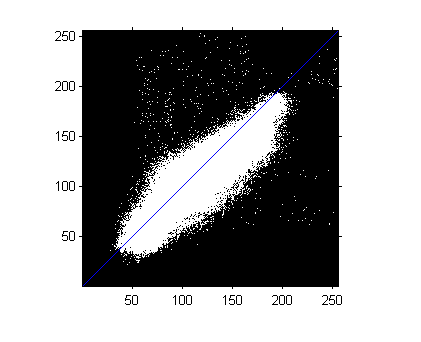
\includegraphics[width=0.45\textwidth]{Fig/compareintensities.png}
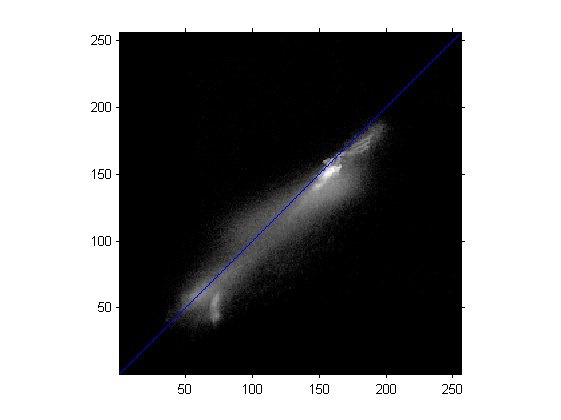
\includegraphics[width=0.45\textwidth]{Fig/compareintensities_log.png}
\caption{Courbes d'intensités comparées. Sur l'image de gauche, chaque point $(x,y)$ blanc correspond à l'existence d'un couple dont l'intensité est $x$ sur une image et $y$ sur l'autre. A droite, le nombre de points correspondant est sommé et passé en échelle logarithmique. En bleu, la droite d'équation $y=x$. Les points s'éloignant fortement de cet axe sont probablement des points présentant des reflets.}
\label{itensitecompare}
\end{figure}
Ces courbes d'intensité montrent la complexité du problème ; même recalées, les images présentent des variations locales importantes d'intensité (la droite a une forte épaisseur). Ainsi, il est difficile de catégoriser les points présentant des reflets. La fonction $f$ doit donc prendre en compte tous les points. La moyenne arithmétique \\
Dans la section~\ref{fusionmin}, nous proposons une fusion par minimum sur chaque canal de couleur. Nous proposons ensuite des fusions par médiane ; elle se fait par canal RGB dans la section~\ref{fusionmediane}, par médiane vectorielle dans la section~\ref{fusiontruemediane}, ou par une méthode légèrement différente dans un autre espace de couleur, détaillée dans la section~\ref{fusionlab}.\\
Il est également possible de travailler dans l'espace gradient au lieu de l'espace de l'image. Dans ce cas, l'image fusionnée J est définie par
\[
\nabla J(x,y)=f\left(\nabla \tilde I_1(x,y), ..., \nabla \tilde I_n(x,y)\right)
\]
Ce cas est détaillé dans la section~\ref{fusiongrad}. Les résultats obtenus par ces méthodes sont comparées dans la section~\ref{results}.
%------------------------------------------------------------> SUB SUB SECTION Fusion par minimum
\subsubsection{Fusion par minimum}
\label{fusionmin}
Pour cette méthode, nous faisons l'hypothèse que les reflets ne font qu'ajouter de la luminosité aux différents pixels de l'image, et que les reflets ne peuvent se retrouver dans toutes les images. Dès lors, il suffit de prendre le minimum de chaque canal de couleur pour parvenir à éliminer les reflets. En notant $R$, $G$ et $B$ les canaux de couleurs, on écrit
\[
J(x,y,c)=\min_{i=1..N}\tilde I_i(x,y,c) \quad \forall c \in \{R,G,B\}
\]
Cette méthode, bien que simple, élimine très efficacement les reflets lambertiens. Elle présente cependant le désavantage de donner des couleurs non naturelles, c'est-à-dire qu'elle ne garantit pas que les pixels de l'image $J$ ainsi obtenue proviennent des images d'origine. De plus, il est attendu que cette méthode assombrisse les images ; en particulier, d'éventuelles ombres se verront assez nettement avec cette méthode.
%------------------------------------------------------------> SUB SUB SECTION Fusion par médianne vectorielle
\subsubsection{Fusion par médiane car canal}
\label{fusionmediane}
Un autre choix possible pour la fonction est la médiane :
\[
J(x,y,c)=\underset{i=1..N}{\mathrm{median}}\tilde I_i(x,y,c) \quad \forall c \in \{R,G,B\}
\]
Ici, l'hypothèse faite est que les reflets se retrouvent sur moins de la moitié des pixels considérés. Elle est donc plus forte que l'hypothèse de la section précédente ; en particulier, cette méthode est inadaptée si une majorité des prises de vue sont semblables. Cependant, elle est plus robuste à des données très différentes des autres. 
\subsubsection{Fusion par médiane vectorielle}
\label{fusiontruemediane}
La méthode précédente présente le désavantage de mélanger les canaux couleurs d'images différentes, ce qui peut conduire à des couleurs non naturelles. Pour pallier à ce problème, nous avons également implémenté un équivalent de la médiane dans l'espace vectoriel des couleurs, appelée "médiane vectorielle". En notant $(\mathbf{x}_i)_{i \in I}$ une liste de vecteurs, elle est définie par
\[
\mathrm{vecmedian}\left((\mathbf{x}_i)_{i \in I}\right) = \underset{i \in I}{\mathrm{argmin}} \sum_{j \in I} ||\mathbf{x}_i-\mathbf{x}_j||_1
\]
La norme $L_1$ est ici utilisée. Il est possible de vérifier que cette médiane est identique à la médiane classique lorsque le nombre de dimensions est 1. \\
Ainsi, pour la fonction $f$ que nous choisissons est ici la fonction vecteur median :
\[
J(x,y)=\mathrm{vecmedian}\left(\tilde I_1(x,y), ..., \tilde I_n(x,y)\right)
\]
En toute rigueur, le vecteur médian n'est pas toujours défini. Il est possible en effet que plusieurs vecteurs $\mathbf{x}$ atteignent le minimum de la définition. En pratique, nous prenons soin de toujours sélectionner des vecteurs provenant de la même image en cas de conflit entre deux images ; ainsi, il n'y a pas de discontinuité dans l'image résultante liée à ce problème. Dans le cadre de la médiane canal par canal, si le nombre d'images est pair, nous utilisons la moyenne des deux scalaires pouvant convenir.
\subsubsection{Fusion par médiane dans l'espace Lab}
\label{fusionlab}
%------------------------------------------------------------> SUB SUB SECTION Fusion dans l'espace gradient
\subsubsection{Fusion dans l'espace gradient}
\centering
\label{fusiongrad}
Enfin, une méthode décrite dans~\citep{haro2012photographing} permettant de réduire plus les reflets consiste à prendre la médiane vectorielle dans l'espace gradient des images. Dans un premier temps, chaque image recalée $\tilde I$ est convertie en niveau de gris $tilde I^g$. Nous calculons ensuite le gradient de chacune de ces images. Nous en construisons une carte d'index, définie par
\[
a(i,j) = arg\underset{k}{\mathrm{vecmedian}}\nabla\tilde I_k(i,j)
\]
Cette carte nous sert à construire le gradient de l'image résultante en chaque canal :
\[
F(x,y,c) = \tilde \nabla I_{a(i,j)}(x,y,c)
\]
Pour chaque canal de couleur $c$, nous reconstruisons l'image $J$ qui devrait être telle que
\[
\nabla J(x,y,c) = F(x,y,c)
\]
Cependant, il est important de noter ici que $F$ n'est pas réellement le gradient d'une image, et, par conséquent, il est impossible de résoudre cette équation. Nous nous efforcerons de fait de minimiser
\[
||\nabla J - F||
\]
L'équation de Poisson s'écrit
\[
\Delta J = \div F
\]
c'est-à-dire, en chaque point,
\[
J(i+1,j)+J(i-1,j)+J(i,j+1)+J(i,j-1)-4J(i,j)=F(i,j)
\]
Pour la résoudre, nous procédons par une méthode itérative. Nous initialisons $J$ par
\[J_0 = \tilde I_1\]
et nous répétons, jusqu'à convergence, l'équation
\[
J_{n+1}(i,j) = \frac{1}{4}J_n(i+1,j)+J_n(i-1,j)+J_n(i,j+1)+J_n(i,j-1)-F(i,j)
\]
En pratique, une douzaine d'itérations suffit pour éliminer les reflets. Cependant, le système ne converge pas car $\div F$ n'est pas réellement un Laplacien. De fait, nous observons des zones d'instabilité assez marquées, qui détruisent progressivement l'image. Ces zones naissent plus rapidement aux endroits où le recalage d'images est perfectible. De fait, 
, et nous en calculons la médiane vectorielle en chaque point. Ensuite, nous construisons les gradients de chaque canal de couleur de l'image fusionnée en prenant, pour chaque point et chaque canal, le gradient de l'image dont la médiane est issue. Ce sont donc bien les gradients des canaux de couleurs qui sont considérés.\\
Lorsque l'on connait le gradient $F$ d'une image, il est possible de la retrouver en minimisant $\min||\mathrm{grad}I - F||$. Ceci se fait grâce à l'équation de Poisson $\Delta I = \mathrm{div}F$. Cette équation est alors résolue, canal par canal, en passant par la transformée de Fourier, s'inspirant de~\citep{morel2010pde}. Rencontrant des difficultés dans cette dernière étape, nous n'avons pas pu terminer cette méthode. Elle donne cependant d'excellents résultats dans~\citep{haro2012photographing}, éliminant certains reflets apparaissant dans une majorité d'images (voir figure~\ref{poissonfig}).
\begin{figure}
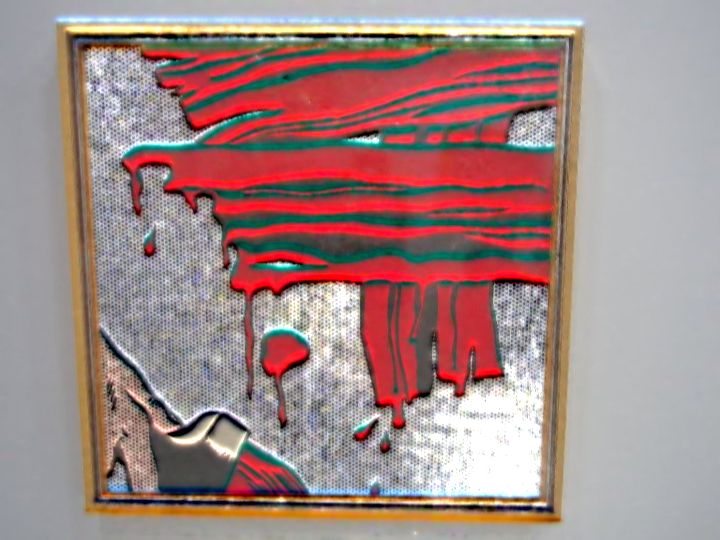
\includegraphics[width=0.6\textwidth]{Fig/poisson.png}
\caption{Image fusionnée obtenue par la méthode des gradients médians. On aperçoit des zones saturées (blanches et noires) qui correspondent à des divergences dans la résolution de l'équation de Poisson. Ces zones correspondent aux zones où le recalage est imparfait.}
\label{poissonfig}
\end{figure}
%------------------------------------------> SECTION Implémentation
\section{Implémentation}

\subsection{Choix technique}
Nous avons implémenté la méthode décrite dans l'article à l'aide du language C++ accompagné de la librarie OpenCV~\citep{opencv_library} de traitement d'image. Cette librarie, très utilisée dans l'industrie, permet d'accélerer le traitement d'image et met à disposition de l'utilisateur plusieurs fonctions (comme par exemple l'algorithme de RANSAC, implémenté dans la fonction \texttt{findHomography}).

\subsection{Architecture}
La méthode décrite ci-dessus est fortement dépendante des paramètres d'entrées et des images à traiter. Par exemple, sur certaines images, la méthode de fusion par minimum est plus adaptée que la méthode de fusion par médianne. Il est donc nécessaire de permettre à l'utilisateur de sélectionner les différentes techniques de recalage et de fusion d'image. Ainsi, nous avons séparé les différente responsabilités entre plusieurs fichiers et classes. Plusieurs méthodes(situées dans les fichiers \texttt{ImageFitter} \texttt{ImageMerger}) permettent de sélectionner les différentes techniques possibles. 

\subsection{Collaboration}
La collaboration a été réalisé grâce au gestionnaire de version git. La totalité du code et ses révisions antérieures sont donc disponible sur Github : http://github.com/jcaille/CVCanvas

%------------------------------------------> SECTION Résultats
\section{Résultats}
\label{results}
Les résultats varient peu selon les méthodes (figure~\ref{mediane}). Les médianes permettent de retirer de nombreux artéfacts de reflets, mais ne fonctionnent pas là où une majorité d'images présentent des artéfacts. Les méthodes de médiane, canal par canal ou globale, donnent les mêmes résultats sur les exemples que nous avons essayés.
\begin{figure}
\centering
\begin{minipage}{0.6\linewidth}
% 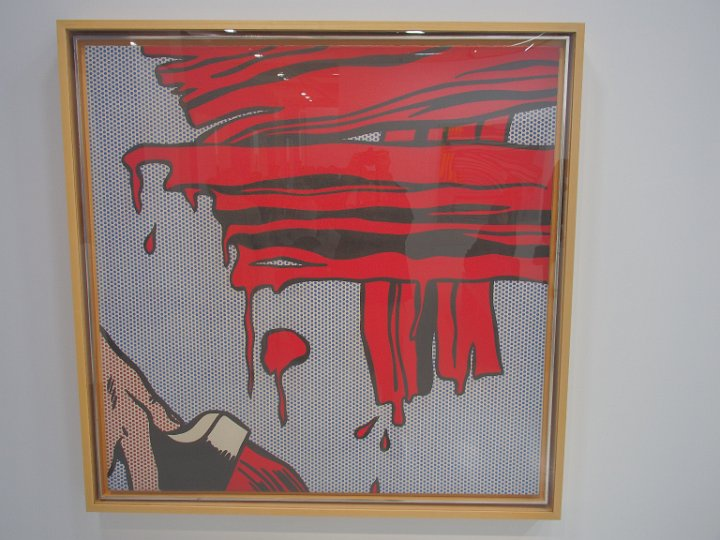
\includegraphics[width=\textwidth]{Fig/reference.jpg}
\end{minipage}
\begin{minipage}{0.6\linewidth}
% 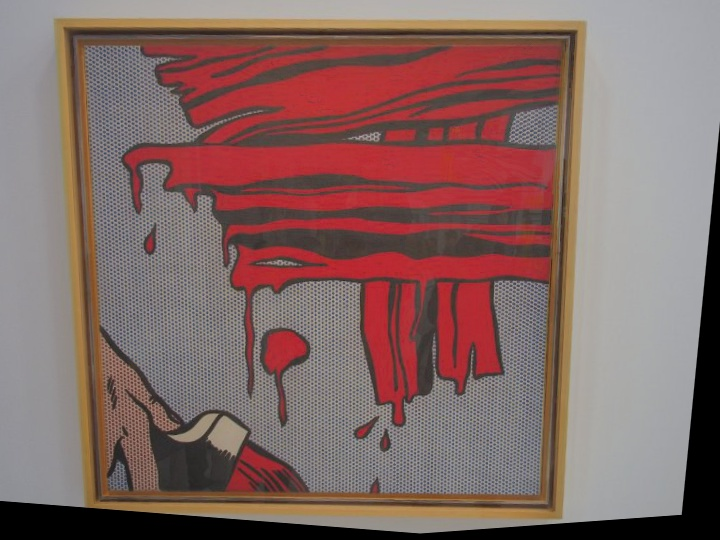
\includegraphics[width=\textwidth]{Fig/merge_min.jpg}
\end{minipage}
\begin{minipage}{0.6\linewidth}
% 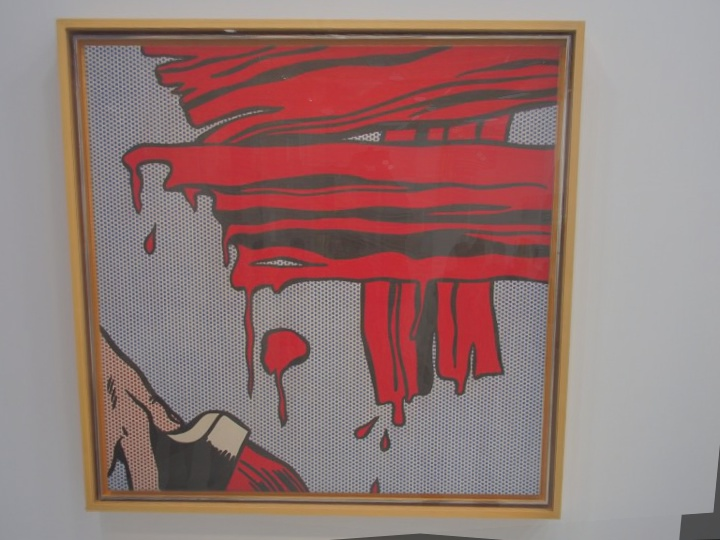
\includegraphics[width=\textwidth]{Fig/merge_median.jpg}
\end{minipage}
\caption{Correction des artéfacts. De haut en bas : image de référence, puis corrigée avec les méthodes du minimum et de la médiane.}
\label{mediane}
\end{figure} 
%------------------------------------------> SECTION Améliorations possibles
\section{Améliorations possibles}

Plusieurs amélioration de l'algorithme sont envisageables. Si les images obtenues sont de bonne qualité, l'algorithme ne sait pas faire la différence entre les zones de la peinture et les zones extérieures (cadre, mur, paysage, ...), dans lesquelles la fusion est effectuée alors qu'elle n'a pas de sens. Une possibilité pour détecter ces zones et de segmenter l'image de référence (par exemple en utilisant des snakes quadrangulaires) entre un "intérieur" sur lequel la fusion serait effectué et un extérieur sur lequel on garderait le contenu d'origine. Pour s'aider dans cette segmentation, nous pourrions utiliser les informations des autres photos du tableau.

De plus, l'algorithme que nous avons développé (en particulier la partie de fusion) n'est pas de fait résistant aux changements de contrastes en général. Une idée pour corriger ce défaut serait d'égaliser les histogrammes les différentes images (de préférence en limitant cette égalisation à la zone "intérieur" du tableau).
\bibliographystyle{plain}
\bibliography{QUEEN}
\end{document}
